
%!TEX ROOT=slehokri_bp.tex


\chapter{STM32 microcontrollers}
\label{chap:STM}
\section{Indroduction}
\label{sec:stm_intro}
STM32 is a family of 32-bit microcontrollers by STMicroelectronics based on ARM Cortex-M processor, namely Cortex-M3, Cortex-M4(F), Cortex-M0, Cortex-M0+, Cortex-M7F, and Cortex-M33F. The STM32 family consists of numerous series of microcontrollers designed for various use-cases. These can be divided into four main groups: Mainstream, High Performance, Ultra-low-power, and Wireless series. As every series has specific features and peripherals, I will only focus on the main differences between used ARM Cortex cores. Table \ref{tab:cortex} shows the utilization of ARM cores in the particular STM32 series.
\begin{table}[ht]
\begin{ctucolortab}
\begin{tabular}{cc}
\bfseries ARM Core & \bfseries STM32 series \\\Midrule
Cortex-M3 & F1, F2, L1 \\ 
Cortex-M4F & F3, F4, G4, L4, L4+, WB, WL\tablefootnote{Based only on ARM Cortex-M4 (without FPU).} \\	
Cortex-M0 & F0 \\ 
Cortex-M0+ & G0, L0 \\
Cortex-M7F & F7, H7 \\
Cortex-M33F & L5, U5
\end{tabular}
\end{ctucolortab}
\caption{ARM Core utilization in STM32 family}
\label{tab:cortex}
\end{table}

\section{Division by ARM cores}
\label{sec:stm_arm_division}
	\subsection{Cortex-M3}
	\label{sub:stm_m3}
Cortex-M3 was the first processor in the Cortex-M generation and the first core used in the STM32 family in the STM32F1 series of microcontrollers. ARM first released this high-performance processor based on ARMv7-M architecture in 2005. It features modified Harvard architecture (with unified memory space) and a 3-stage pipeline. Thanks to 32-bit addressing, 4GB of memory space is supported.
	
	\subsection{Cortex-M4F}
	\label{sub:stm_m4}
The successor to Cortex-M3 was released by ARM in 2010. This new generation called Cortex-M4 is similar to its predecessor in design and features. The instruction set now contains DSP (Digital Signal Processor) instructions for more complex data processing, and there is an optional single-precision FPU (Floating Point Unit). Variant with FPU is known as Cortex-M4F. 
	
	\subsection{Cortex-M0}
	\label{sub:stm_m0}		%TODO citace?
Cortex-M0 processor is one of the smallest ARM processors available, optimized for small size and low power consumption \cite{m0_web}. The processor is based on ARMv6-M with a smaller instruction set, uses Von Neumann architecture, and has a 3-stage pipeline. This small core is ideal for general data processing tasks, where low cost and high energy efficiency matter.
	
	\subsection{Cortex-M0+}
	\label{sub:stm_m0_plus}
Cortex-M0+ is based on Cortex-M0, thus adopting small size and further improving power efficiency and performance. The instruction set and tools are fully backward compatible with Cortex-M0. ARM reduced pipeline to 2 stages to lower power consumption. Furthermore, the processor has more options available, such as vector table relocation and memory protection unit (MPU).
	
	\subsection{Cortex-M7F}
	\label{sub:stm_m7}
The most powerful processor in the Cortex-M family is Cortex-M7. The processor uses ARMv7-M architecture and features the longest pipeline with six stages. Given the used architecture, the instruction set contains DSP instructions, and there is also an optional FPU, which can be single-precision or even double-precision. Main buses have been enlarged to 64-bit wide. Variant with FPU is known as Cortex-M7F. 
	
	\subsection{Cortex-M33F}
	\label{sub:stm_m33}
Cortex-M33 is the newest core used in the STM32 family of microcontrollers. The processor is based on more recent ARMv8-M architecture with Harvard bus architecture. It is conceptually similar to Cortex-M4 with a 3-stage pipeline and optional single-precision FPU. The core is ideal for IoT applications as it has optional TrustZone security instructions for hardware-enforced isolation and memory protection unit (MPU). Variant with FPU is known as Cortex-M33F. 

\section{Architecture}
\label{sec:stm_arch}
The ARM itself does not make microcontrollers but instead designs the core and other components and licenses them to silicon designers. It is the same concept with the STM32 family of microcontrollers - ST Microelectronics obtains the processor design from ARM as a base for their microcontroller. The company then attaches its own set of memories and peripherals, such as ADC (Analog-to-Digital converter), DAC (Digital-to-Analog converter), clock generation and timers, and various types of connectivity peripherals like UART, SPI, I2C, etc.

This approach is depicted in figure \ref{fig:f303}, where there is a circuit diagram of the STM32F303CC microcontroller that I will use in my project.  You can see a Cortex-M4F processor with all the ST-specific peripherals and memories around.
\begin{figure}
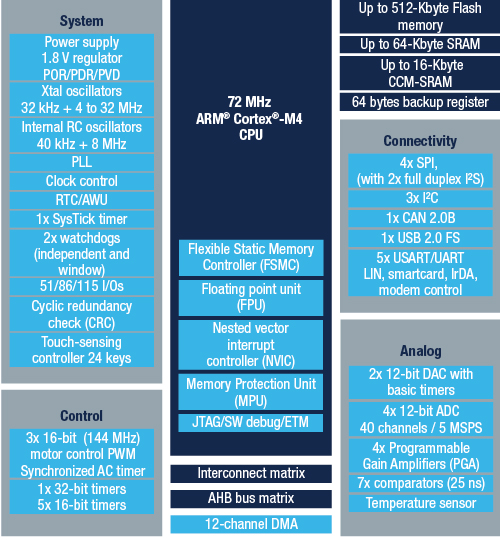
\includegraphics[width=0.6\linewidth]{figures/en.bd_stm32f303}
\caption{STM32F303 circuit diagram \cite{f303_diagram}} %TODO citace - web ST
\label{fig:f303}
\end{figure}

	\subsection{Clock}
	\label{sub:clock}
The frequency of the processor, buses, and connected peripherals is derived from their clock source, usually an oscillator. STM32 microcontrollers include internal clock sources, or it is possible to connect external clock sources. The frequency from other clock sources can be multiplied by the internal PLL (Phase-Locked Loop) circuit to speed up the microcontroller further and reach higher frequencies. Several prescalers allow finetuning bus and peripherals speed. Internal clock sources have the advantage of providing a clock source at a low cost with no external components. But being an RC oscillator, the frequency produced is usually not as accurate as an external oscillator.

	\subsection{Interrupts}
	\label{sub:nvic}
The main controller responsible for handling interrupt events is Nested Vectored Interrupt Controller, NVIC for short. It is tightly coupled to the Cortex core allowing for low latency interrupt processing. The NVIC features support for up to 240 interrupt inputs with programmable priorities, which can be individually enabled or disabled, along with Non-Maskable Interrupts (NMI). Furthermore, in the case of Cortex M3 and M4, the interrupt latency is only 12 cycles with zero wait state memory \cite{yu}. All interrupts can be triggered by software by writing to the appropriate register; this also applies to many system exceptions. Microcontroller vendors determine the total number of interrupts supported by a device with Cortex core when designing the chip.

In the  STM32 family of microcontrollers, there is also a hardware device called extended interrupts and events controller (EXTI). This controller is connected to the NVIC and supports up to 36 external/internal interrupt events. Active edge for external interrupts is programmable. With this device, it is possible to generate interrupts or wake-up events from external peripherals and GPIO pins.

	\subsection{Buses}
	\label{sub:buses}
The Cortex core has a well-defined on-chip bus structure and protocol that allows the connection of various memory configurations and peripherals. Since most of the Cortex cores use Harvard architecture, multiple bus interfaces enable simultaneous access to instructions and data. Buses are (most of the time) 32-bit wide.

The primary bus interface protocol utilized is AHB Lite (Advanced High-performance Bus). This pipelined protocol allows high operation frequency with a small silicon footprint and is used in program memory and system bus interfaces. Usually, the bus can have more devices that act as a master, for example, DMA (Direct Memory Acces) or Ethernet controller. Therefore the processor includes a bus matrix (or AHB interconnect matrix) that manages transfers from multiple bus masters to different slave segments. Particular bus matrix implementation is shown in figure \ref{fig:f303_busmatrix}.
\begin{figure}
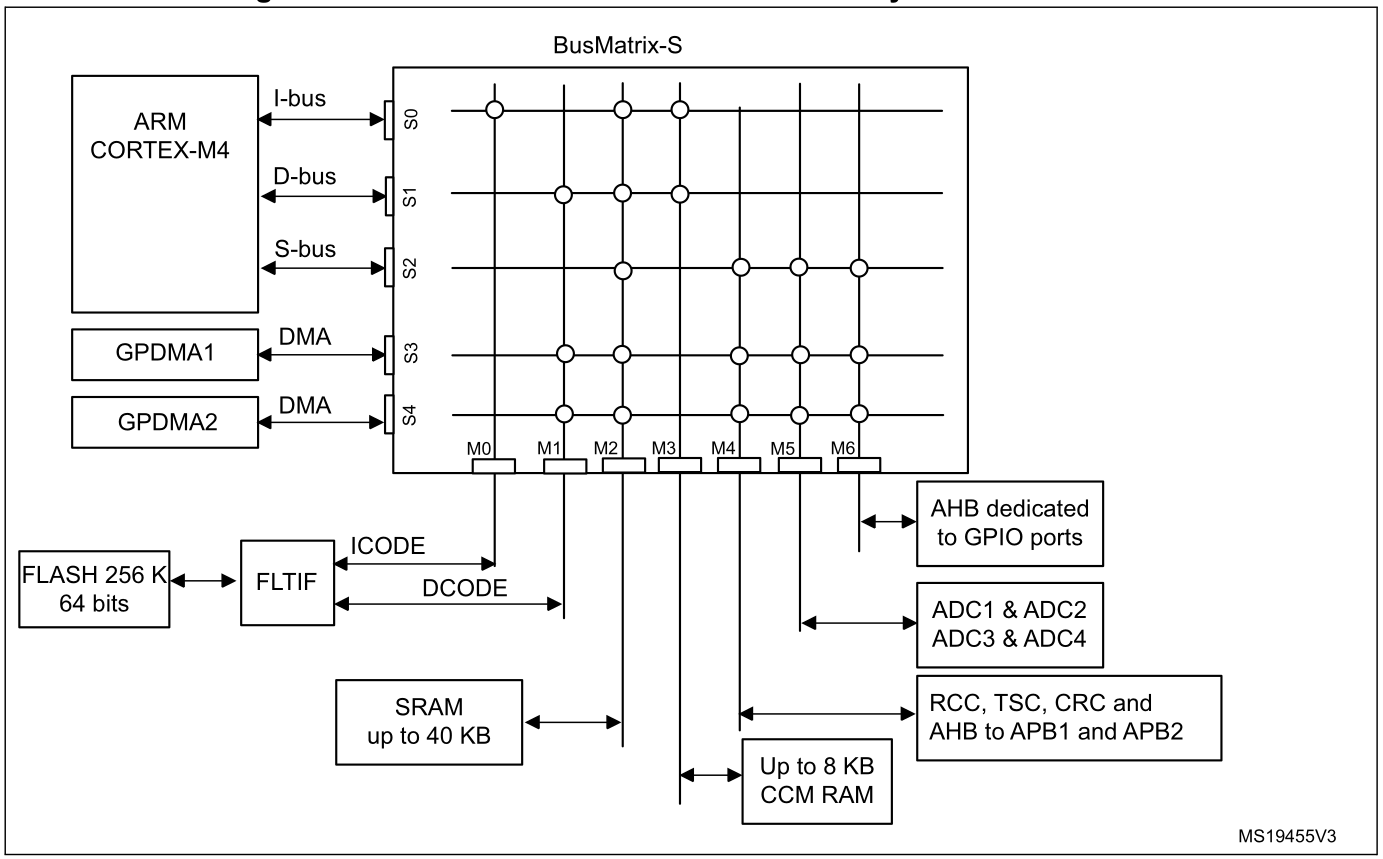
\includegraphics[width=0.7\linewidth]{figures/f303_bus_matrix}
\caption{STM32F303CC bus architecture \cite{f303_ref}} %TODO citace - referencak F303
\label{fig:f303_busmatrix}
\end{figure}

The secondary bus used mainly for connecting peripherals is APB (Advanced Peripheral Bus). Usually, APB buses are connected to the AHB bus matrix using bridge components. If the peripheral needs higher bandwidth and operation speed, for example, the ADC, it is possible to connect it to the faster AHB bus.

Some of the more advanced Cortex processors also use other buses. For example, the Cortex-M7 has an additional 64-bit wide AXI bus that can be used for faster FLASH memory access. 

	\subsection{Memories}
	\label{sub:memories}
Thanks to the bus architecture, different memories can easily be attached to the AHB bus with suitable memory interface logic. Even though the bus is 32-bit, there are no width restrictions if appropriate conversion hardware is used.

Usually, types like SRAM and FLASH are often used for data memory and program code memory, respectively. However, there is no real limitation on memory type connected to a processor, and different technologies can be utilized, e.g., SDRAM, EPROM, etc. Also, memory size is not limited. The only requirement is that the memory should be byte-addressable, and the interface has to support byte, half-word, and word transfers.

	\subsection{Direct Memory Acces (DMA)}
	\label{sub:dma}
A Direct Memory Access is a programmable hardware unit connected to the AHB bus. It reduces processor load by offloading memory transfer operations. Supported transfer directions are peripheral-to-peripheral, memory-to-peripheral, peripheral-to-memory, and also memory-to-memory. There is a small overhead when setting the unit, but afterward, the whole transfer is handled by DMA without processor intervention, thus leaving computing power to other tasks. The unit usually has several independent channels with assignable priorities.


\section{Peripherals}
\label{sec:stm_periph}
Every series of STM32 microcontrollers features different peripherals, from the basic ones with little settings to more advanced and configurable ones. This section is not supposed to be an overly exhausting listing of all the peripherals across all STM32 families, but instead, I would like to focus mainly on the most used ones and those I use in my project.

	\subsection{GPIO}
	\label{sub:gpio}
The abbreviation GPIO stands for General-Purpose Input/Output. It is a designation for microcontroller pins. The pins are arranged in groups of sixteen and are referred to as GPIOx (for example, GPIOA, GPIOC). Not every pin from the group has to be physically present. Especially for microcontrollers with smaller packages, it is common that some pins from the group are missing. In figure \ref{fig:gpio}, there is a typical internal structure of the GPIO pin with internal protection diodes.

Each pin can be set as either input, output, or alternate function. Internal pull-up and pull-down resistors are available as well. These features are configured and controlled by software. Most GPIO control registers are 32-bit and have to be accessed as 32-bit words, although some STM32 series support half-word and byte access.

If the pin is in alternate function mode, it is controlled by a connected peripheral, for example, ADC, timer, USART, etc. Thanks to the highly flexible pin multiplexing, many peripheral functions can be remapped to another pin. Debug pins are in alternate function mode by default after microcontroller reset. Other pins are usually in floating input mode.

When the pin is set as output or alternate function, it can be push-pull or open-drain. Most of the pins can provide $\pm20 \text{ mA}$ of current, making it possible to drive, for example, a LED directly. However, the total current that a microcontroller can source or sink is limited. It is not advised to connect pins to voltages higher than the supply voltage; yet, many pins are 5V tolerant.
\begin{figure}
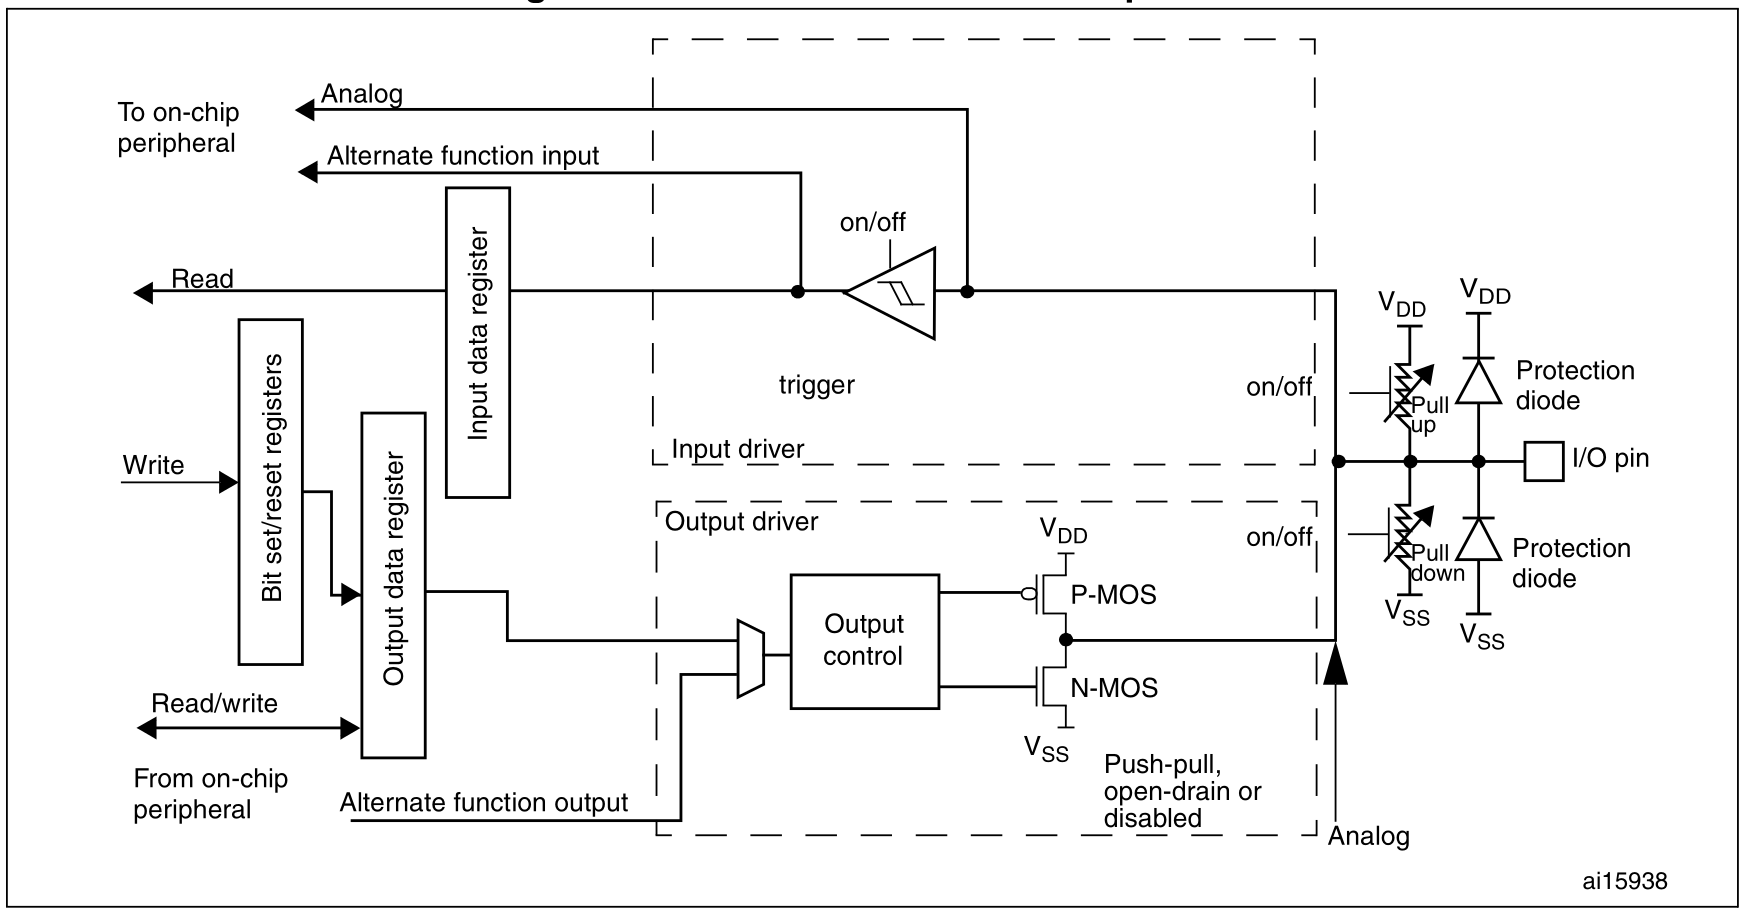
\includegraphics[width=0.9\linewidth]{figures/io_port}
\caption{Basic structure of an I/O port bit \cite{f303_ref}} %TODO citace - referencak F303
\label{fig:gpio}
\end{figure}

	\subsection{Timers}
	\label{sub:timers}
Timers are one of the basic peripherals. The primary function is counting; it can measure time and do a specific action, for example, toggle a pin. The counter clock frequency is adjustable using a programmable prescaler. Usually, there are many timers in the microcontroller with varying features.

The simplest ones are basic timers. These timers are predominantly used for time-base generation as they feature only a simple up counter, usually 16-bit.

The more feature-rich timers are general-purpose timers. With those, besides the basic functionality, it is possible to generate various waveforms or measure the pulse length of the input signal. Furthermore, there can be support for incremental encoders with quadrature output, which can then be connected straight to the MCU. I found this feature very useful as interfacing encoders this way is pretty straightforward.

As the name suggests, the advanced-control timers are the most advanced. Functionality includes all the features of previously mentioned timers with some added or upgraded. Most of the time, advanced-control timers have more channels that can be synchronized together or using an external signal. This ability makes it possible to generate a three-phase PWM output to control a three-phase motor like BLDC.

The Cortex core contains another 24-bit timer called SysTick timer, dedicated to real-time operating systems. It usually provides OS with regular timer interrupts for time-keeping, but it can also be used as a standard down counting timer.

	\subsection{Analog-to-Digital Converter (ADC)}
	\label{sub:adc}
Another common peripheral is the Analog-to-Digital converter. This peripheral can convert a given voltage (usually between 0V and analog-reference voltage) to a binary number. One possible utilization can be reading a potentiometer voltage to obtain the trigger position.

The particular implementation can vary between the STM32 series, but most of the time, they use successive-approximation ADC or Sigma-Delta ADC. It can be configured to measure either single-ended input or differential input in continuous or single-shot mode. Also, some internal channels are available, for example, connected to an internal temperature sensor and voltage reference.

An internal ADC self-calibration is a convenient feature that can compensate for offset and gain error and significantly improve conversion accuracy. The calibration is triggered by software. If the application has to handle a large amount of data, the DMA unit can serve the ADC memory transfers to free the CPU. Moreover, an analog watchdog feature can monitor the converted voltage and generate an interrupt if it exceeds the programmed thresholds. 

	\subsection{Digital-to-Analog Converter (DAC)}
	\label{sub:dac}
The Digital-to-Analog converter does the exact opposite of the Analog-to-Digital converter. It converts the given binary number to a corresponding analog voltage. It is possible to generate complex waveforms or an audio signal with this peripheral. The DAC can therefore be used in many audio applications. If at least two channels are available, the conversion can be independent or simultaneous with external triggers, providing the ability to generate a stereo audio signal. Usually, the DAC also features a noise-wave generation or a triangular-wave generation. Such as with the ADC, the DAC memory transfers can be controlled by DMA, thus freeing up the CPU.

	\subsection{Serial Peripheral Interface (SPI)}
	\label{sub:spi}
The serial peripheral interface is a master-slave interface bus used to communicate with smaller devices, such as sensors, memories, displays, LED drivers, etc. If supported by a particular microcontroller, the peripheral can also be configured as an I2S (Inter-Integrated Sound) interface, allowing the connection of digital audio devices.

Peripheral settings are rich to support a wide range of compatible devices. It can operate either as a master, providing a clock to connected devices, or as a slave; multimaster mode is also possible. Communication mode and speed can be configured as well as frame size and clock polarity. The DMA unit can help handle a lot of data and achieve high data communication rates with hardware control. Moreover, the SPI peripheral includes a hardware CRC unit with automatic CRC error checking. This feature can be useful when communicating with SD memory cards.

	\subsection{Inter-Integrated Circuit (I2C)}
	\label{sub:i2c}
The Inter-Integrated Circuit is another commonly used short-range communication bus in embedded systems. It is also a synchronous interface that requires fewer communication wires than SPI but provides lower communication rates. As the SPI interface, the I2C can be used to communicate with small displays, memories, and other rather lower-speed devices.

The peripheral supports both 7-bit and 10-bit addressing modes, programmable analog and digital noise filters, and configurable multiple speed modes depending on the particular microcontroller. Furthermore, the peripheral includes a hardware CRC unit, and it is designed to support SMBus and PMBus protocol used by PCs and servers. DMA channel connecting I2C is also available to provide hardware control of transfers.

	\subsection{USART}
	\label{sub:usart}
USART stands for Universal Synchronous/Asynchronous Receiver/Transmitter. Although computers are rarely equipped with serial ports these days, serial communication is still highly used in the embedded world as it is simple and easy to use. This peripheral is flexible and has a wide range of applications - it can be used for simple UART communication; in the synchronous mode, it can act like SPI master/slave; it also features hardware management of some signals from industry standards like RS-232 and RS-485. Moreover, there is support for Smartcard communication, IrDA serial infrared communication, and multiprocessor communication. It is also possible to use the peripheral to implement other buses with hardware control, for example, Modbus or 1-Wire.  

The peripheral offers many programmable parameters like baud rate, data word length, the number of stop bits, data order, parity control, oversampling, etc. Furthermore, USART is the source of many interrupts indicating various statuses and flags. The peripheral is connected to the DMA unit like other serial communication peripherals, significantly facilitating handling continuous streams or huge amounts of data.